\documentclass[tikz,border=4pt]{standalone}
% Paleta y fuentes compartidas por el libro y las figuras (única fuente de verdad).
\RequirePackage{xcolor}
\definecolor{oxido}{HTML}{B7410E}
\definecolor{cobre}{HTML}{D27D2D}
\definecolor{carbon}{HTML}{2B2B2B}
\definecolor{azul}{HTML}{1F5F8B}
\definecolor{arena}{HTML}{F4EDE4}

\usepackage{fontspec}
\setsansfont{FiraSans}[Extension=.otf,UprightFont=*-Regular,BoldFont=*-Bold,ItalicFont=*-Italic,BoldItalicFont=*-BoldItalic]
\setmonofont{FiraMono}[Extension=.otf,UprightFont=*-Regular,BoldFont=*-Medium]
\usetikzlibrary{positioning,arrows.meta,calc,fit}
\begin{document}
\sffamily\small
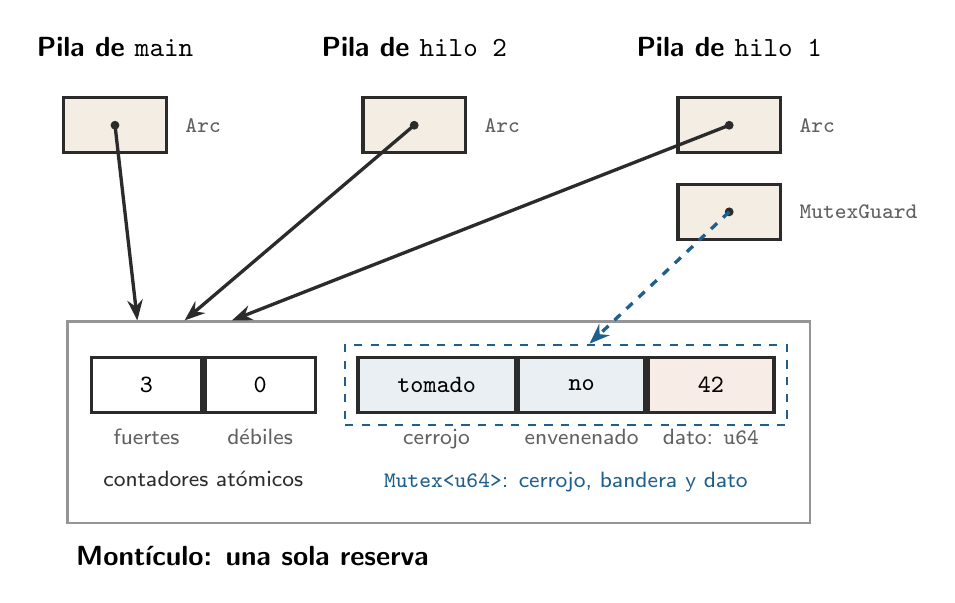
\begin{tikzpicture}[
  celda/.style={draw=carbon,minimum height=7mm,minimum width=13mm,font=\ttfamily\small,fill=white,very thick},
  rotulo/.style={font=\sffamily\footnotesize\color{carbon!75}},
  >={Stealth[length=2.6mm]}]
  % Tres pilas: una por hilo
  \foreach \n/\x/\k in {main/0/0,hilo 2/3.8/2,hilo 1/7.8/1} {
    \node[font=\sffamily\bfseries] at (\x,1.0) {Pila de \texttt{\n}};
    \node[celda,fill=arena] (p\k) at (\x,0) {};
    \node[rotulo,anchor=west] at ($(p\k.east)+(0.1,0)$) {\texttt{Arc}};
    \fill[carbon] (p\k.center) circle (1.6pt);
  }
  % guarda del hilo 1, debajo de su Arc
  \node[celda,fill=arena] (g) at (7.8,-1.1) {};
  \fill[carbon] (g.center) circle (1.6pt);
  \node[rotulo,anchor=west] at ($(g.east)+(0.1,0)$) {\texttt{MutexGuard}};
  % Bloque del montículo
  \node[celda,minimum width=14mm] (f) at (0.4,-3.3) {3};
  \node[celda,minimum width=14mm,anchor=west] (d) at (f.east) {0};
  \node[celda,minimum width=20mm,anchor=west,fill=azul!10] (c) at ($(d.east)+(0.5,0)$) {tomado};
  \node[celda,minimum width=16mm,anchor=west,fill=azul!10] (e) at (c.east) {no};
  \node[celda,minimum width=16mm,anchor=west,fill=oxido!10] (v) at (e.east) {42};
  \node[rotulo,below=2pt of f] (lf) {fuertes};
  \node[rotulo,below=2pt of d] {débiles};
  \node[rotulo,below=2pt of c] {cerrojo};
  \node[rotulo,below=2pt of e] {envenenado};
  \node[rotulo,below=2pt of v] {dato: \texttt{u64}};
  \node[draw=azul,thick,dashed,inner sep=4pt,fit=(c)(v)] (mx) {};
  \node[font=\sffamily\footnotesize,text=azul,anchor=north] (lm) at ($(mx.south)+(0,-0.45)$) {\texttt{Mutex<u64>}: cerrojo, bandera y dato};
  \node[font=\sffamily\footnotesize,text=carbon,anchor=north] (lc) at ($(f.south)!0.5!(d.south)+(0,-0.6)$) {contadores atómicos};
  \node[draw=carbon!50,thick,inner sep=8pt,fit=(f)(v)(mx)(lm)(lc)] (bloque) {};
  \node[font=\sffamily\bfseries,anchor=north west] at ($(bloque.south west)+(0,-0.15)$) {Montículo: una sola reserva};
  % Flechas
  \draw[->,very thick,carbon] (p0.center) -- ($(bloque.north west)+(0.9,0)$);
  \draw[->,very thick,carbon] (p2.center) -- ($(bloque.north west)+(1.5,0)$);
  \draw[->,very thick,carbon] (p1.center) -- ($(bloque.north west)+(2.1,0)$);
  \draw[->,very thick,azul,dashed] (g.center) -- ($(mx.north)+(0.3,0)$);
\end{tikzpicture}
\end{document}
